%----------------------------------------------------------------------------------------
%	SLIDE 5./4.
%----------------------------------------------------------------------------------------
\begin{frame}
\frametitle{Processes during a simulation}

\begin{block}{}
	\begin{itemize}
		\item With different \texttt{physics list} we'll obtain different results (again)
		\item We can study the energy deposit and occurrence of physical processes individually
	\end{itemize}
\end{block}

\begin{figure}
	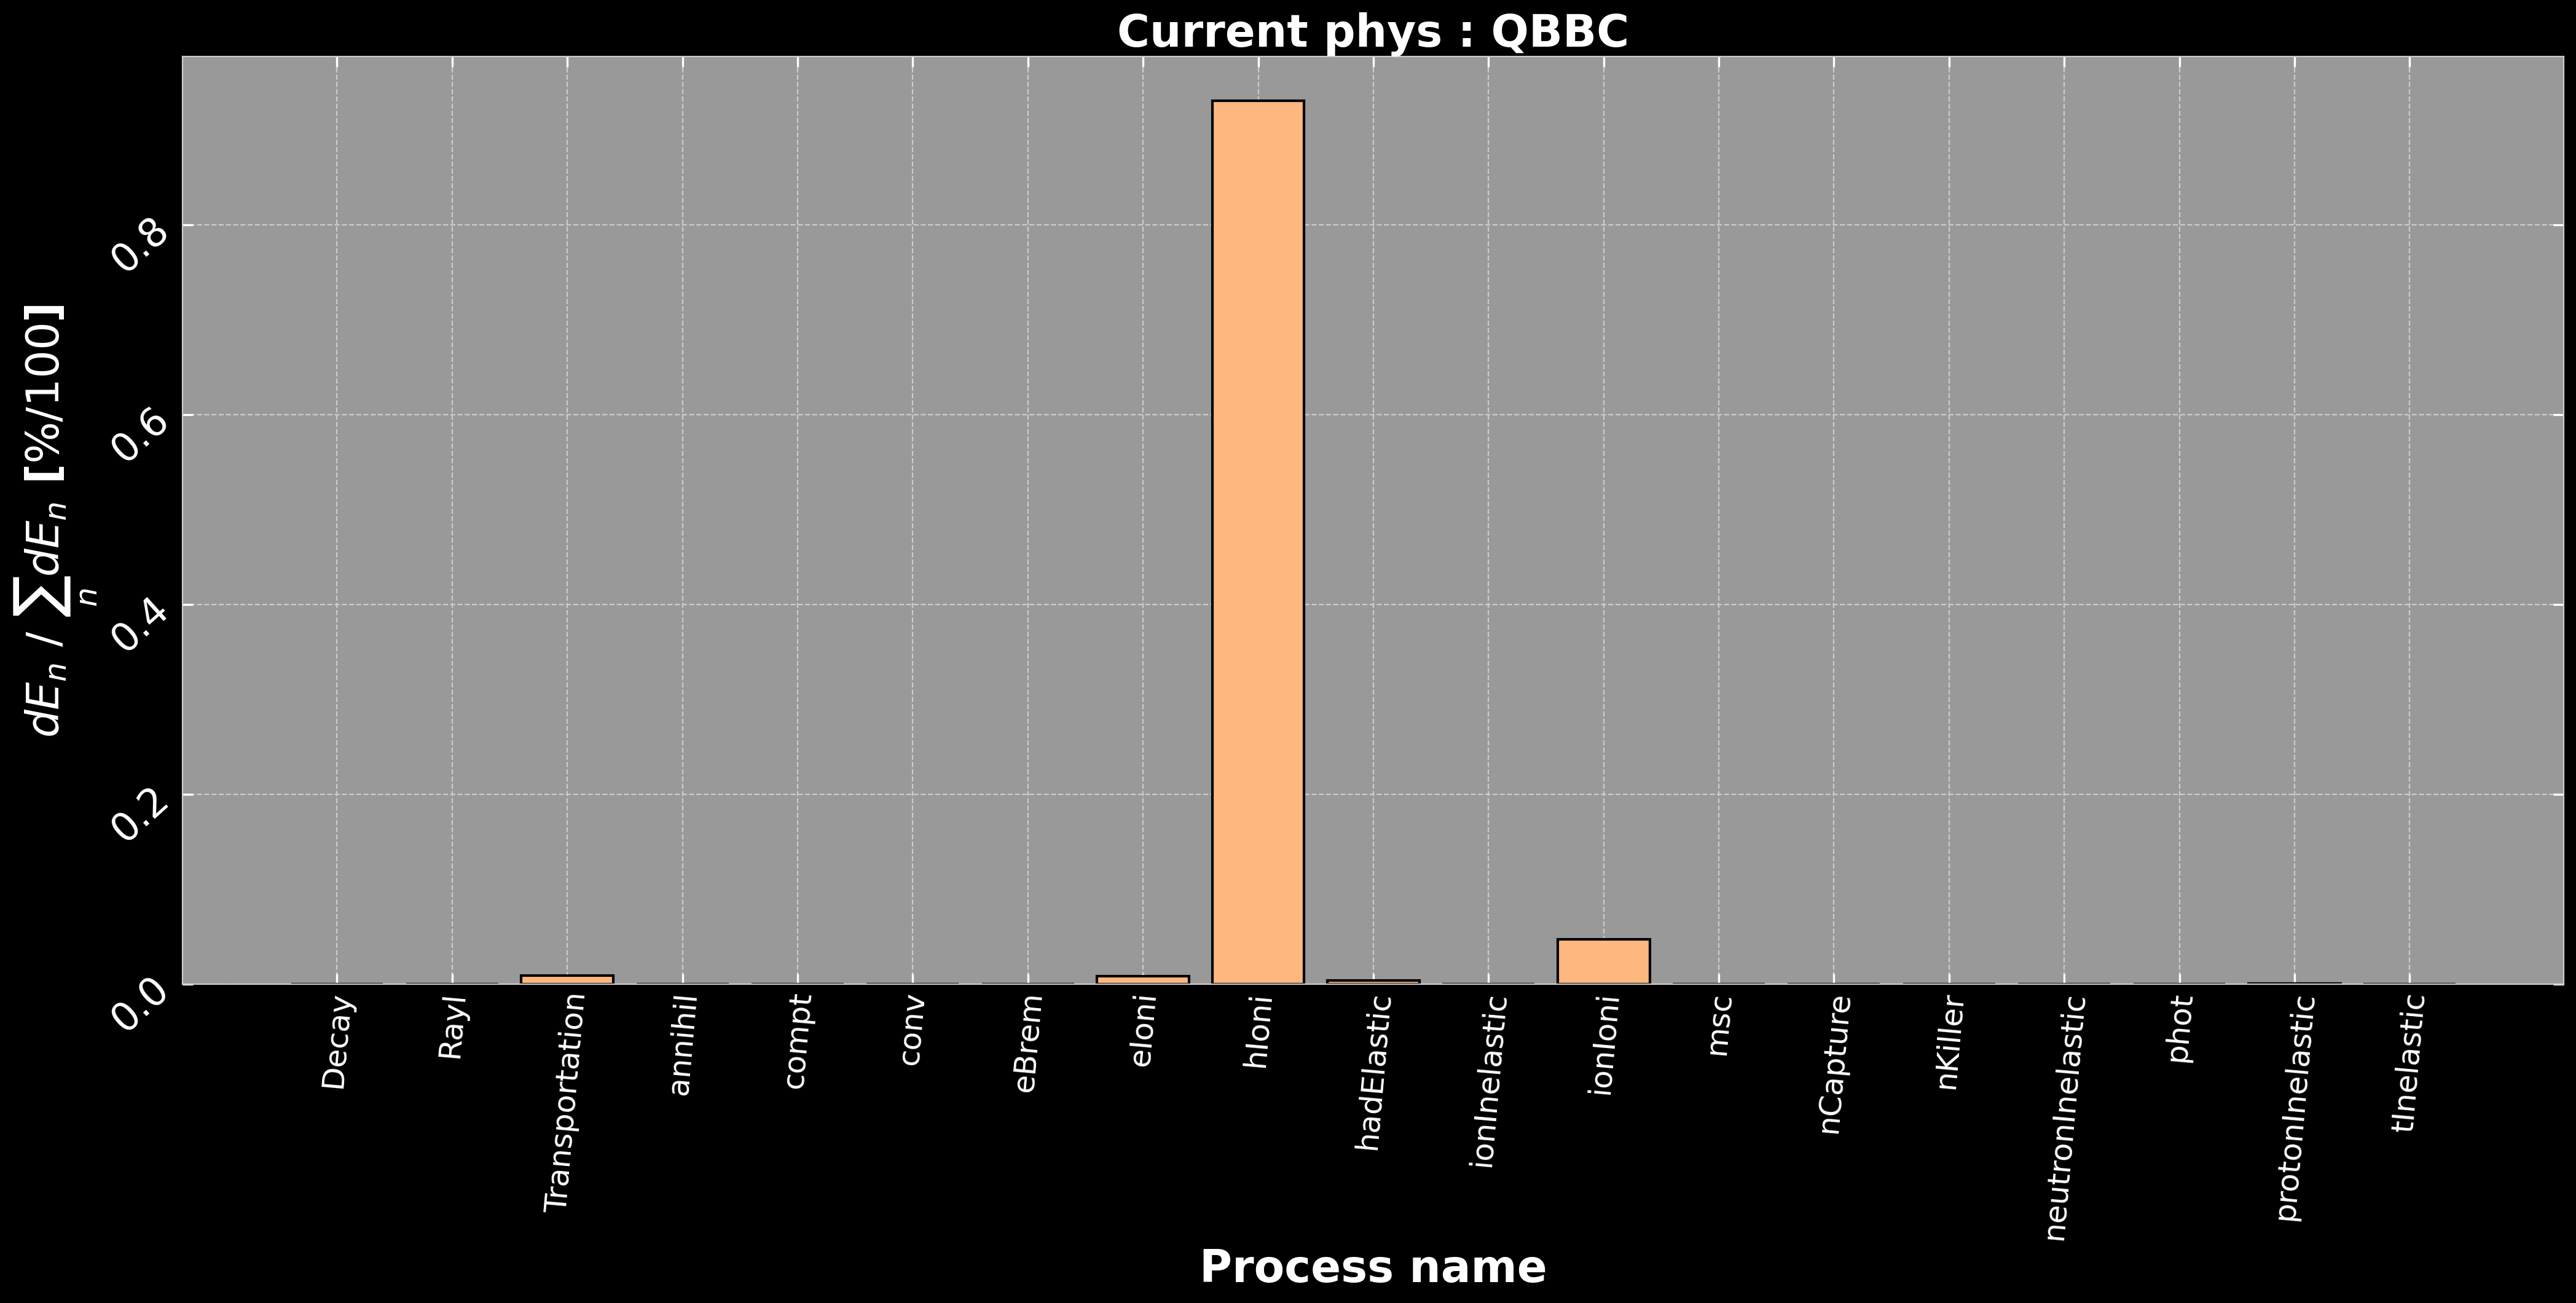
\includegraphics[width=0.8\textwidth]{images/process_dist_weighted_E100_phQBBC.png}
\end{figure}

\end{frame}